\subsection{Support vector machines}

While the origins of support vector machines (SVMs) are old (and go back to \cite{vapnik1963pattern}), their modern treatment was initiated in \cite{boser1992training} and \cite{cortes1995support} (binary classification) and \cite{drucker1997support} (regression). We refer to \href{http://www.kernel-machines.org/books}{http://www.kernel-machines.org/books} for an exhaustive bibliography on their theoretical and empirical properties. SVMs have been very popular since their creation among the machine learning community. Nonetheless, other tools (neural networks especially) have gained popularity and progressively replaced SVMs in many applications like computer vision notably.

\subsubsection{SVM for classification}

As is often the case in machine learning, it is easier to explain a complex tool through an illustration with binary classification. In fact, sometimes, it is originally how the tool was designed (e.g., for the perceptron). Let us consider a simple example in the plane, that is, with two features. In Figure~\ref{svmscheme}, the goal is to find a model that correctly classifies points: filled circles versus empty squares.

\begin{figure}[!htbp]
\centering
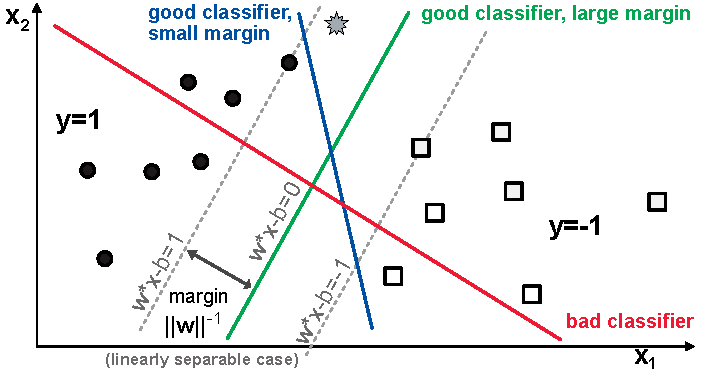
\includegraphics[width=0.625\linewidth]{files/svm-803b09e4fc2fd0cb8220fad1b82ec088.pdf}
\caption[]{Diagram of binary classification with support vectors.}
\label{svmscheme}
\end{figure}

A model consists of two weights $\textbf{w}=(w_1,w_2)$ that load on the variables and create a natural linear separation in the plane. In the example above, we show three separations. The red one is not a good classifier because there are circles and squares above and beneath it. The blue line is a good classifier: all circles are to its left and all squares to its right. Likewise, the green line achieves a perfect classification score. Yet, there is a notable difference between the two.

The grey star at the top of the graph is a mystery point and given its location, if the data pattern holds, it should be a circle. The blue model fails to recognize it as such while the green one succeeds. The interesting features of the scheme are those that we have not mentioned yet, that is, the grey dotted lines. These lines represent the no-man's land in which no observation falls when the green model is enforced. In this area, each strip above and below the green line can be viewed as a margin of error for the model. Typically, the grey star is located inside this margin.

The two margins are computed as the parallel lines that maximize the distance between the model and the closest points that are correctly classified (on both sides). These points are called \textbf{support vectors}, which justifies the name of the technique. Obviously, the green model has a greater margin than the blue one. The core idea of SVMs is to maximize the margin, under the constraint that the classifier does not make any mistake. Said differently, SVMs try to pick the most robust model among all those that yield a correct classification.

More formally, if we numerically define circles as +1 and squares as -1, any `good' linear model is expected to satisfy:

\begin{equation}
\label{eq:svm0}
\left\{\begin{array}{lll}
\sum_{k=1}^Kw_kx_{i,k}+b \ge +1 & \text{ when } y_i=+1 \\
\sum_{k=1}^Kw_kx_{i,k}+b \le -1 & \text{ when } y_i=-1,
\end{array}\right.
\end{equation}

which can be summarized in compact form $y_i \times \left(\sum_{k=1}^K w_kx_{i,k}+b \right)\ge 1$. Now, the margin between the green model and a support vector on the dashed grey line is equal to $||\textbf{w}||^{ -1}=\left(\sum_{k=1}^Kw_k^2\right)^{ -1/2}$. This value comes from the fact that the distance between a point $(x_0,y_0)$ and a line parametrized by $ax+by+c=0$ is equal to $d=\frac{|ax_0+by_0+c|}{\sqrt{a^2+b^2}}$. In the case of the model defined above \ref{eq:svm0}, the numerator is equal to 1 and the norm is that of $\textbf{w}$. Thus, the final problem is the following:

\begin{equation}
\label{eq:svm1}
\underset{\textbf{w}, b}{\text{argmin}} \ \frac{1}{2} ||\textbf{w}||^2 \ \text{ s.t. } y_i\left(\sum_{k=1}^Kw_kx_{i,k}+b \right)\ge 1.
\end{equation}

The dual form of this program (see chapter 5 in \cite{boyd2004convex}) is

\begin{equation}
\label{eq:svm1b}
L(\textbf{w},b,\boldsymbol{\lambda})=
 \frac{1}{2}||\textbf{w}||^2 + \sum_{i=1}^I\lambda_i\left(y_i\left(\sum_{k=1}^Kw_kx_{i,k}+b \right)- 1\right),
\end{equation}

where either $\lambda_i=0$ or $y_i\left(\sum_{k=1}^Kw_kx_{i,k}+b \right)= 1$. Thus, only some points will matter in the solution (the so-called support vectors). The first order conditions impose that the derivatives of this Lagrangian be null:

\begin{equation}
\frac{\partial L}{\partial \textbf{w}}L(\textbf{w},b,\boldsymbol{\lambda})=\textbf{0}, \quad \frac{\partial L}{\partial b}L(\textbf{w},b,\boldsymbol{\lambda})=0,
\end{equation}

where the first condition leads to

\begin{equation}
\textbf{w}^*=\sum_{i=1}^I\lambda_iu_i\textbf{x}_i.
\end{equation}

This solution is indeed a linear form of the features, but only some points are taken into account. They are those for which the inequalities \ref{eq:svm0} are equalities.

Naturally, this problem becomes infeasible whenever the condition cannot be satisfied, that is, when a simple line cannot perfectly separate the labels, no matter the choice of coefficients. This is the most common configuration and datasets are then called logically \textit{not linearly separable}. This complicates the process but it is possible to resort to a trick. The idea is to introduce some flexbility in \ref{eq:svm0} by adding correction variables that allow the conditions to be met:

\begin{equation}
\label{eq:svm2}
\left\{\begin{array}{lll}
\sum_{k=1}^Kw_kx_{i,k}+b \ge +1-\xi_i & \text{ when } y_i=+1 \\
\sum_{k=1}^Kw_kx_{i,k}+b \le -1+\xi_i & \text{ when } y_i=-1,
\end{array}\right.
\end{equation}

where the novelties, the $\xi_i$ are positive so-called \textbf{`slack' variables} that make the conditions feasible. They are illustrated in Figure~\ref{svmscheme2}. In this new configuration, there is no simple linear model that can perfectly discriminate between the two classes.

\begin{figure}[!htbp]
\centering
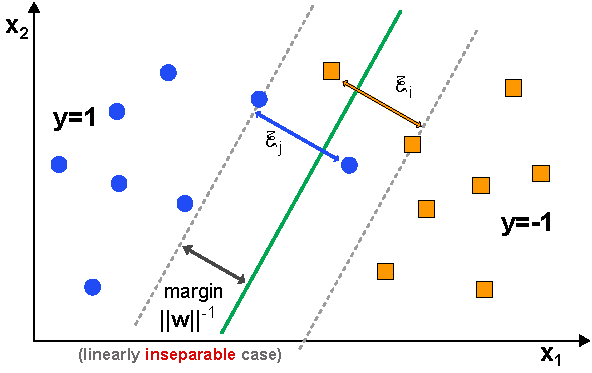
\includegraphics[width=0.625\linewidth]{files/svm2-f652c58a89424e044dacced0d8e3d5b6.pdf}
\caption[]{Diagram of binary classification with SVM - linearly inseparable data.}
\label{svmscheme2}
\end{figure}

The optimization program then becomes

\begin{equation}
\label{eq:svm3}
\underset{\textbf{w},b, \boldsymbol{\xi}}{\text{argmin}} \ \frac{1}{2} ||\textbf{w}||^2+C\sum_{i=1}^I\xi_i \ \text{ s.t. } \left\{ y_i\left(\sum_{k=1}^Kw_k\phi(x_{i,k})+b \right)\ge 1-\xi_i \ \text{ and } \ \xi_i\ge 0, \ \forall i  \right\},
\end{equation}

where the parameter $C>0$ tunes the cost of mis-classification: as $C$ increases, errors become more penalizing.

In addition, the program can be generalized to nonlinear models, via the kernel $\phi$ which is applied to the input points $x_{i,k}$. Nonlinear kernels can help cope with patterns that are more complex than straight lines (see Figure~\ref{svmscheme4}). Common kernels can be polynomial, radial or sigmoid. The solution is found using more or less standard techniques for constrained quadratic programs. Once the weights $\textbf{w}$ and bias $b$ are set via training, a prediction for a new vector $\textbf{x}_j$ is simply made by computing $\sum_{k=1}^Kw_k\phi(x_{j,k})+b$ and choosing the class based on the sign of the expression.

\begin{figure}[!htbp]
\centering
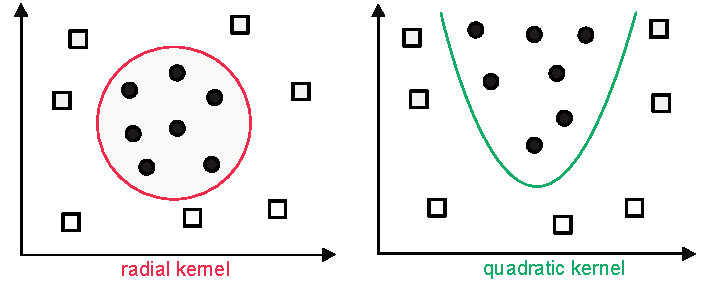
\includegraphics[width=0.5\linewidth]{files/kernel-c4ceac2655372255245b865b96528581.pdf}
\caption[]{Examples of nonlinear kernels.}
\label{svmscheme4}
\end{figure}

\subsubsection{SVM for regression}

The ideas of classification SVM can be transposed to regression exercises but the role of the margin is different. One general formulation is the following

\begin{equation}
\label{eq:svm4}
\begin{aligned}
\underset{\textbf{w},b, \boldsymbol{\xi}}{\text{argmin}} \  & \frac{1}{2} ||\textbf{w}||^2+C\sum_{i=1}^I\left(\xi_i+\xi_i^* \right)\\
 \text{ s.t. }&  \sum_{k=1}^Kw_k\phi(x_{i,k})+b -y_i\le \epsilon+\xi_i \\
&  y_i-\sum_{k=1}^Kw_k\phi(x_{i,k})-b \le \epsilon+\xi_i^* \\
&\xi_i,\xi_i^*\ge 0, \ \forall i  ,
\end{aligned}
\end{equation}

and it is illustrated in Figure~\ref{svmscheme3}. The user specifies a \textbf{margin} $\epsilon$ and the model will try to find the linear (up to kernel transformation) relationship between the labels $y_i$ and the input $\textbf{x}_i$. Just as in the classification task, if the data points are inside the strip, the slack variables $\xi_i$ and $\xi_i^*$ are set to zero. When the points violate the threshold, the objective function (first line of the code) is penalized. Note that setting a large $\epsilon$ leaves room for more error. Once the model has been trained, a prediction for $\textbf{x}_j$ is simply $\sum_{k=1}^Kw_k\phi(x_{j,k})+b$.

\begin{figure}[!htbp]
\centering
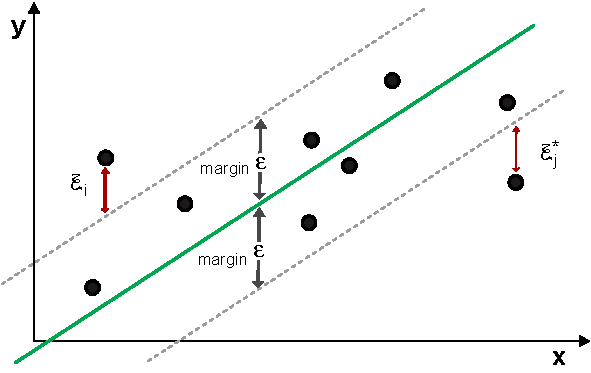
\includegraphics[width=0.625\linewidth]{files/svm3-f19cc71e59b778ccb6f885d525a469b0.pdf}
\caption[]{Diagram of regression SVM.}
\label{svmscheme3}
\end{figure}

Let us take a step back and simplify what the algorithm does, that is: minimize the sum of squared weights $||\textbf{w}||^2$ subject to the error being small enough (modulo a slack variable). In spirit, this somewhat the opposite of the penalized linear regressions which seek to minimize the error, subject to the weights being small enough.

The models laid out in this section are a preview of the universe of SVM engines and several other formulations have been developed. One reference library that is coded in C and C++ is \textbf{LIBSVM} and it is widely used by many other programming languages. The interested reader can have a look at the corresponding article \cite{chang2011libsvm} for more details on the SVM zoo (a more recent November 2019 version is also available online).

\subsubsection{Practice}

In Python, the LIBSVM library is exploited in scikit-learn through the \texttt{sklearn.svm} module. This provides both \texttt{SVR} (Support Vector Regression) and \texttt{SVC} (Support Vector Classification).

In the implementation of LIBSVM, the package requires to specify the label and features separately. For this reason, we recycle the variables used for the boosted trees. Moreover, the training being slow, we perform it on a subsample of these sets (first thousand instances).

\begin{verbatim}
from sklearn.svm import SVR
import numpy as np
import pandas as pd
import matplotlib.pyplot as plt
import seaborn as sns
import warnings
warnings.filterwarnings('ignore')
plt.style.use('seaborn-v0_8-whitegrid')
sns.set_palette("husl")

# Building the data & import functions
from data_build import generate_data
data_ml, features, features_short, returns, stock_ids, stock_ids_short = generate_data()
features_short =["Div_yld", "EPS", "size_avg_252d", "mom_252", "OCF_Growth_1Y", "PB", "vol_252"]
separation_date = "2017-01-15"

data_ml_clean = data_ml.dropna(subset=(features_short + ['R1M']))
training_sample = data_ml_clean[data_ml['date'] <= separation_date]
testing_sample = data_ml_clean[data_ml['date'] > separation_date]  #
\end{verbatim}

\begin{verbatim}
# Fit SVM for regression
fit_svm = SVR(
    kernel='rbf',        # SVM kernel (or: 'linear', 'poly', 'sigmoid')
    epsilon=0.1,         # Width of strip for errors
    gamma=0.5,           # Constant in the radial kernel
    C=0.1                # Slack variable penalisation
)

X_train = training_sample[features_short].iloc[0:1000]
y_train = training_sample['R1M'].iloc[0:1000]

# Train on first 1001 instances
fit_svm.fit(
    X_train,     # Training features
    y_train      # Training labels
)
\end{verbatim}

\begin{verbatim}
SVR(C=0.1, gamma=0.5)
\end{verbatim}

\begin{verbatim}
# Select test features
test_feat_short = testing_sample[features_short]

# Predictions
predictions = fit_svm.predict(test_feat_short)

# MSE
mse = np.mean((predictions - testing_sample['R1M'])**2)
print(f"MSE: {np.round(mse,5)}")

# Hit ratio
hit_ratio = np.mean(predictions * testing_sample['R1M'] > 0)
print(f"Hit ratio: {np.round(hit_ratio,5)}")
\end{verbatim}

\begin{verbatim}
MSE: 0.01591
Hit ratio: 0.52338
\end{verbatim}

The results are slightly better than those of the boosted trees. All parameters are completely arbitrary, especially the choice of the kernel. We finally turn to a classification example.

\begin{verbatim}
from sklearn.svm import SVC

# Fit SVM for classification
fit_svm_C = SVC(
    kernel='sigmoid',    # SVM kernel
    gamma=0.5,           # Parameter in the sigmoid kernel
    coef0=0.3,           # Parameter in the sigmoid kernel
    C=0.2                # Slack variable penalisation
)

# Train on first 1000 instances
fit_svm_C.fit(
    training_sample[features].iloc[:1000],     # Training features
    training_sample['R1M_C'].iloc[:1000]       # Training labels (classification)
)

# Accuracy
accuracy = np.mean(
    fit_svm_C.predict(testing_sample[features]) == testing_sample['R1M_C']
)
print(f"Accuracy: {np.round(accuracy,5)}")
\end{verbatim}

\begin{verbatim}
Accuracy: 0.49979
\end{verbatim}

Both the small training sample and the arbitrariness in our choice of the parameters may explain why the predictive accuracy is so poor.

\subsubsection{Coding exercises}

\begin{enumerate}
\item From the simple example shown above, extend SVM models to other kernels and discuss the impact on the fit.
\item Train a vanilla SVM model with labels being the 12-month forward (i.e., future) return and evaluate it on the testing sample. Do the same with a simple random forest. Compare.
\end{enumerate}